\documentclass{article} % For LaTeX2e
\usepackage{iclr2027_conference,times}
\usepackage{kotex} % Added for Korean output (remove later if necessary)
\usepackage{booktabs}
\usepackage{graphicx}
\usepackage{amsmath}
\usepackage{algorithm}
\usepackage{algorithmic}
\input{math_commands.tex}

\usepackage{hyperref}
\usepackage{url}
\usepackage{color}

% 빈칸(TODO)을 쉽게 찾을 수 있도록 강조하는 매크로
\newcommand{\todo}[1]{\textcolor{red}{\textbf{[TODO: #1]}}}

\title{Amplifying Exploitation in Visual Reinforcement Learning through Episodic Retrieval}

\author{\todo{Author 1 Name} \\
\todo{Author 1 Affiliation} \\
\texttt{\todo{Author 1 Email}} \\
\And
\todo{Author 2 Name} \\
\todo{Author 2 Affiliation} \\
\texttt{\todo{Author 2 Email}} \\
% 필요한 만큼 \And 로 추가하세요
}

\newcommand{\fix}{\marginpar{FIX}}
\newcommand{\new}{\marginpar{NEW}}

%\iclrfinalcopy % Uncomment for camera-ready version, but NOT for submission.
\begin{document}

\maketitle

\begin{abstract}
Recent advancements in Reinforcement Learning (RL) have heavily adopted Diffusion-based models to improve visual representations, but they suffer from prohibitive computational costs. In this paper, we investigate whether this heavy generative approach is the only solution. While prior work assumes that compact visual representations discard fine-grained details, we revisit this assumption. Our probing experiments show that lightweight encoders can retain substantial task-relevant information despite poor visual reconstruction. These findings suggest that poor reconstruction alone does not establish the absence of task-relevant information, motivating interventions that improve how downstream Actor-Critic learners use the available representations. Building on this, we demonstrate that augmenting the Actor-Critic optimization process is a highly effective way to distinguish aliased states. To this end, we propose FLASH (Fast Latent Anchor Search with Hashing), an efficient retrieval module that implicitly supports Actor-Critic learning by selecting anchors based on a surprise score and augmenting training batches with these anchors and structurally similar past experiences. By improving downstream discrimination between aliased states, FLASH acts as a versatile plug-and-play module that improves the overall performance of the evaluated baselines without altering their underlying encoders, confirming that heavy generative models are not strictly necessary and acting as a powerful exploitation amplifier.
For STORM, FLASH increases total wall-clock training time over 100,000 environment steps by 5.11--7.41\% across the three evaluated GPUs.
\end{abstract}

\section{Introduction}
\label{sec:intro}

Recent high-fidelity generative world models demonstrate that preserving visual detail can improve control, but this comes with increased computation \citep{lee2026edeline, alonso2024diffusion}. We investigate a complementary question: \textit{Can downstream policy and value optimization make better use of task-relevant information retained in compact visual representations, without requiring heavier generative models?}

Our investigation is motivated by preliminary DRAMA runs on Seaquest: under the same training configuration, we observed scores of approximately 600 and 1,500. In the inspected behavior, the higher-scoring run sustained hunting until oxygen depletion, whereas the lower-scoring run died in collisions during hunting; neither exhibited surfacing with collected divers. This observation suggests that a lightweight encoder architecture can support different levels of performance without observed success in diver-return behavior, motivating investigation of how downstream learning uses available experience. We describe this preliminary observation and its interpretation limits in Appendix~\ref{sec:appendix_ac_bottleneck}.

Although compact visual representations may fail to reconstruct fine-grained visual details, poor reconstruction alone does not establish that task-relevant information has been lost. Our probing experiments show that lightweight encoders can retain substantial task-relevant information despite poor visual reconstruction. In particular, supervised probes predict the evaluated task variables from latent states with high accuracy under clean observations, although probing performance degrades under background corruption. These results motivate exploring downstream optimization as an additional intervention point, without assuming that all task-relevant information is preserved. Specifically, we show that augmenting the Actor-Critic optimization process can help distinguish aliased states, without requiring any changes to the encoder itself.

We use \textit{aliasing} to describe task-relevant differences between states that are difficult for a downstream learner to distinguish in highly similar latent representations; identical latent vectors are not required. We use \textit{blurry} only to describe the visual appearance of decoded images.

Accurate prediction by a supervised probe, however, does not guarantee effective use of the same information for control: a supervised probe and an Actor-Critic learner receive different learning signals and optimize different objectives. We therefore investigate whether targeted reuse of informative experiences can help translate successful behavior into policy improvement. FLASH pursues this direction by identifying salient learning events, retrieving structurally similar past experiences through hashing, and incorporating them into the same Actor-Critic training batch. Its design targets the use of experiences already encountered, without assuming that retrieval alone can discover previously unseen rewarding behavior.

Our contributions are threefold:
\begin{itemize}
    \item First, we use diagnostic probing to assess whether lightweight encoder representations retain task-relevant information despite poor visual reconstruction, finding that supervised probes predict selected task variables from latent states with high accuracy under clean observations.
    \item Second, motivated by this evidence, we investigate downstream Actor-Critic optimization as a way to better utilize the available representations without replacing the encoder with a heavier model.
    \item Finally, we propose FLASH, a plug-and-play retrieval mechanism that groups structurally similar past experiences within the same Actor-Critic training batch, without modifying the underlying encoder architecture. On Atari 100k, FLASH improves the IQM human-normalized score of \todo{evaluated baselines} by \todo{relative IQM improvement}, with a measured total training time increase of 5.11--7.41\% for STORM across three GPUs (Table~\ref{tab:efficiency}).
\end{itemize}

\section{Related Work}
\label{sec:related}

\textbf{Latent World Models.}
Dreamer and DreamerV2 learn policies through latent imagination \citep{hafner2019dream, hafner2020mastering}, while STORM and DRAMA use Transformer- and Mamba-based dynamics, respectively \citep{zhang2023storm, wang2025drama}. FLASH augments the contexts used for Actor-Critic imagination while retaining the base agent's encoder and world-model architectures.

\todo{First conduct a brief feasibility study of porting FLASH to TWISTER as the third base agent. If the required changes are extensive, use TWM as the alternative. Finalize the third base agent after this assessment.}

\textbf{Representation Learning and Diffusion World Models.}
Prior work improves visual representations through reconstruction \citep{hafner2019learning}, contrastive learning (\citealp{laskin2020curl}), predictive consistency (\citealp{schwarzer2020data}), decoupled representation learning (\citealp{stooke2021decoupling}), or prototypical learning (\citealp{deng2022dreamerpro}). DIAMOND instead uses a diffusion world model to preserve visual detail \citep{alonso2024diffusion}. FLASH investigates better downstream use of compact representations through targeted experience reuse.

\textbf{Episodic Control and Retrieval-Augmented RL.}
MFEC, NEC, and EVA use episodic experience to inform value estimates \citep{blundell2016model, pritzel2017neural, hansen2018fast}; ERLAM and subsequent work further structure memory through associative graphs and state abstraction \citep{zhu2020episodic, li2023neural}. FLASH uses hashing to retrieve contexts around selected anchors and incorporates them into Actor-Critic training batches, acting implicitly through batch composition.

\textbf{Prioritized Experience Replay.}
Experience selection has used TD-error \citep{schaul2015prioritized}, value signals \citep{cao2019high}, curiosity \citep{kauvar2023curious}, sequence priorities \citep{karimpanal2018experience, brittain2019prioritized}, and actor-critic-specific criteria \citep{saglam2023actor}. Prioritized Sweeping schedules backups using changes in value estimates \citep{moore1993prioritized}. FLASH selects anchors using a multiplicative score combining TD-error and signed temporal value difference, then retrieves structurally similar contexts for joint training. Appendix~\ref{sec:appendix_related_work} provides further background and comparisons.

\section{Problem Analysis and Motivation}
\label{sec:representation}

\subsection{Reconstruction and Information Loss}
Poor visual reconstruction raises questions about the information available in a model state, but image blurriness alone does not establish information loss. In this section, we investigate whether selected task-relevant variables remain despite poor reconstruction.

As a motivating observation, we note the \textit{temporal persistence of objects} during the \textbf{open-loop imagination phase} in models like DreamerV3 and Drama \citep{hafner2023mastering, wang2025drama}. During this phase, the model predicts future states solely based on its internal transition dynamics, without access to real observations. For instance, in Figure~\ref{fig:temporal_persistence}, the highlighted fish appears less blurry at $t$, more blurry at $t+1$, and less blurry again at $t+2$. This observation suggests that decoded image quality alone is insufficient to assess predictive state information. It does not establish complete information preservation and motivates the direct probing experiments below.

\begin{figure}[!t]
\centering
\begin{minipage}{0.24\textwidth}
  \centering
  \includegraphics[width=\linewidth]{reconstruction/frame_0061_marked.png}\\
  (a) $t$ (less blurry)
\end{minipage}\hspace{0.015\textwidth}%
\begin{minipage}{0.24\textwidth}
  \centering
  \includegraphics[width=\linewidth]{reconstruction/frame_0062_marked.png}\\
  (b) $t+1$ (more blurry)
\end{minipage}\hspace{0.015\textwidth}%
\begin{minipage}{0.24\textwidth}
  \centering
  \includegraphics[width=\linewidth]{reconstruction/frame_0063_marked.png}\\
  (c) $t+2$ (less blurry)
\end{minipage}
\caption{Consecutive decoded frames from an open-loop imagined trajectory. The fish (yellow circles) appears less blurry at $t$ and $t+2$, and more blurry at $t+1$. This observation suggests that decoded image quality alone is insufficient to assess predictive state information; it does not establish complete information preservation.}
\label{fig:temporal_persistence}
\end{figure}

\subsection{Probing the Latent Space}
\label{subsec:probing_latent}
To formally investigate whether standard lightweight encoders successfully capture functionally critical elements, we conducted extensive probing experiments on the Seaquest environment. First, using images with perfectly identical backgrounds varying only the target elements, we observed that the pairwise cosine similarities of latent states encoding different diver counts and positions were strictly less than 1.0 (dropping to $0.86$ and $0.63$, respectively). This suggests sensitivity to changes in these target regions, motivating a direct test of whether a supervised probe can predict the corresponding task variables from latent states.

To assess prediction accuracy, we detached the pre-trained encoder and trained a lightweight MLP to predict ground-truth RAM states (e.g., diver counts and exact $(x, y)$ coordinates) directly from the latent state $z$. As detailed in Appendix \ref{sec:appendix_detailed_probing}, our probing achieved exceptional accuracy ($>99\%$ for diver counting and $92.4\%$ for diver presence prediction) on pristine clean observations.

However, when we injected extreme uniform noise into the background spaces while leaving only the target bounding box intact, the classification accuracy plummeted drastically (e.g., from $99.6\%$ to $68.1\%$ in Seaquest). This drop indicates that the encoder--probe pipeline is sensitive to background corruption. It is consistent with spatial entanglement, but extreme noise also introduces a distribution shift, so this experiment alone does not isolate the cause of the degradation.

Crucially, cosine differences indicate representational sensitivity, whereas the high clean probing accuracy provides more direct evidence that supervised probes can predict the evaluated task variables from the latent states. These findings do not establish that all semantic information is preserved or that spatial entanglement is the sole bottleneck. They nevertheless suggest that poor reconstruction alone is insufficient to diagnose missing task-relevant information, motivating interventions that help downstream learners use the information available in these representations.

\subsection{The Actor-Critic Optimization as an Intervention Point}
\label{subsec:ac_intervention}
Having found that supervised probes can predict selected task-relevant variables from latent states, we investigate whether downstream Actor-Critic optimization can better exploit this available information while retaining the lightweight encoder architecture. Successful prediction by a supervised probe does not establish that policy and value learning will learn to extract or use the same information from reward-driven training signals. This motivates studying the experiences presented to the Actor-Critic as an additional intervention point.

Specifically, FLASH retrieves structurally similar historical experiences around salient learning events and groups them within the same training batch. We hypothesize that this targeted reuse can help the learner distinguish contexts with different return targets and reinforce useful behavior. This is a hypothesis about improving downstream utilization, rather than evidence that Actor-Critic optimization is the sole source of performance limitations.

\section{METHODOLOGY}
\label{sec:method}

FLASH maintains a lightweight episodic memory indexed by Locality-Sensitive Hashing (LSH), selects anchors using a surprise score, and retrieves structurally similar past contexts to augment Actor-Critic training batches. We describe the method in three parts: memory indexing and maintenance (Section~\ref{subsec:flash_memory}), anchor selection and retrieval (Section~\ref{subsec:flash_retrieval}), and integration into Actor-Critic learning (Section~\ref{subsec:flash_learning}). Algorithm~\ref{alg:flash} summarizes the execution order, and Figure~\ref{fig:flash_pipeline} illustrates the overall architecture.

\subsection{Hash-Indexed Episodic Memory}
\label{subsec:flash_memory}

At every environment step, the world model observation encoder and posterior head, jointly denoted by $f_\theta$, map a single observation $o_t$ to a flattened posterior categorical probability vector $z_t = f_\theta(o_t) \in [0,1]^{d}$, where $d = K \times C$ with $K$ categorical variables each of $C$ classes. Specifically, STORM converts posterior logits to probabilities via softmax and applies \textit{unimix} (1\% uniform mixing), yielding $z_t = \operatorname{vec}(0.99\,\operatorname{softmax}(\ell_t) + 0.01/C)$, where $\ell_t \in \mathbb{R}^{K \times C}$ contains the raw posterior logits, softmax is applied over the $C$ classes of each variable, and $K=C=32$. Thus, hashing uses the resulting probabilities, rather than logits or sampled one-hot latent states, and excludes the world model's temporal hidden state. The same probability representation is used for insertion, re-verification, and Global Rebuild. We apply an LSH function $h: \mathbb{R}^d \to \{0,1,\ldots,2^B{-}1\}$ to produce a discrete hash key:
\begin{equation}
h(z_t) = \sum_{i=1}^{B} \mathbf{1}\!\left[\left(W_{\text{proj}}^\top (z_t - \mu)\right)_i > 0\right] \cdot 2^{i-1},
\label{eq:lsh}
\end{equation}
where $B$ is the number of hash bits, $\mu$ is the centering vector (initially $\mathbf{0}$), and $W_{\text{proj}} \in \mathbb{R}^{d \times B}$ is the projection matrix (initially a random Gaussian projection). During \textit{Global Rebuild} (described below), both are updated via PCA on the current buffer's latent distribution to align the hash hyperplanes with the principal axes of variation.

Each transition pointer $(p_t, e)$ (where $p_t$ is the circular buffer index and $e$ is the environment index) is inserted into a hash bucket $\mathcal{B}_{h(z_t)}$. If a pointer's hash key changes (due to Global Rebuild), it is transparently migrated.

\paragraph{Memory Maintenance.}
As the encoder evolves, stored hash keys can become stale. We monitor the average hit rate, defined as the fraction of retrieval candidates passing re-verification (Section~\ref{subsec:flash_retrieval}). If this rate drops below a threshold $\eta$, a \textbf{Global Rebuild} is triggered: all hash buckets are cleared, the PCA projection $W_{\text{proj}}$ and mean $\mu$ are recomputed from a fresh encoding of the entire replay buffer, and all transitions are re-hashed. This refreshes the index to reflect the current representation, subject to a cooldown period to amortize cost.

\subsection{Surprise-Guided Retrieval}
\label{subsec:flash_retrieval}

TD-error magnitude is commonly used as a proxy for how surprising a transition is in prioritized replay \citep{schaul2015prioritized}. In FLASH, \textit{surprise} denotes an anchor-selection score that combines TD-error magnitude with the signed temporal value difference, rather than TD-error magnitude alone. During each world model training step, given a batch of sampled trajectories with value estimates $V(s_t)$ from the critic, we compute:
\begin{align}
\delta_t^{\text{TD}} &= \left| r_t + \gamma \, V(s_{t+1})(1 - d_t) - V(s_t) \right|, \label{eq:td_error} \\
\Delta V_t &= V(s_t) - V(s_{t-1}), \label{eq:value_diff}
\end{align}
where $r_t$ is the reward, $\gamma$ is the discount factor, and $d_t$ is the termination flag. To normalize across environments with varying reward scales, we maintain per-environment exponential moving averages (EMA) of the mean and variance:
\begin{align}
\bar{\mu}_e &\leftarrow (1-\alpha)\bar{\mu}_e + \alpha \cdot \mathbb{E}[\delta^{\text{TD}}_{e}], \quad
\bar{\sigma}^2_e \leftarrow (1-\alpha)\bar{\sigma}^2_e + \alpha \cdot \text{Var}[\delta^{\text{TD}}_{e}], \label{eq:ema_update}
\end{align}
and analogously for $\Delta V$. At each training step, we compute the surprise score $S_u$ using the EMA statistics from preceding batches, then update the statistics with the current batch, including during warmup. The surprise score is:
\begin{equation}
S_t = \text{ReLU}\!\left(\frac{\delta^{\text{TD}}_t - \bar{\mu}_e}{\sqrt{\bar{\sigma}^2_e} + \epsilon}\right) \cdot \text{softplus}\!\left(\frac{\Delta V_t - \bar{\mu}^{V}_e}{\sqrt{\bar{\sigma}^{2,V}_e} + \epsilon}\right).
\label{eq:surprise}
\end{equation}
By pairing a strict ReLU with a softplus, this formulation guarantees that it will never fire unless the TD-error is above average, regardless of how much the value spikes. Conversely, an extremely large TD-error can still trigger the anchor even if the value decreases slightly. This captures precisely the pivotal moments where a highly surprising or high-reward sub-trajectory is first discovered. For each trajectory sequence in the batch, when the maximum surprise score across its time steps exceeds the threshold ($\max_{t \in \text{seq}} S_t > \tau_z$), the corresponding buffer pointer (offset backwards by $\Delta_{\text{anchor}}$ steps to capture the critical preceding actions that caused the surprise; see Appendix~\ref{sec:appendix_causal_anchor} for architectural details) is registered as an \textit{active anchor} $a = (p_{t^*+\Delta_\text{anchor}},\, e)$ where $t^* = \text{argmax}_{t \in \text{seq}} S_t$, in a FIFO queue $\mathcal{A}$.

\paragraph{Neighbor Retrieval and Re-verification.}
At each imagination step (where the agent generates imagined trajectories for policy training), FLASH pops up to $M$ anchors from $\mathcal{A}$. For each anchor $a$ with stored hash key $k_a$, we sample up to $m \times (n{-}1)$ candidate pointers from bucket $\mathcal{B}_{k_a}$ (excluding the anchor itself). To combat \textit{representation drift} (the gradual shift in hash keys as $f_\theta$ evolves), we perform \textbf{lazy re-verification}: each candidate's single-frame observation is re-encoded through the \textit{current} world model, and only candidates whose re-computed hash key matches $k_a$ are retained. This yields a set of verified neighbors $\mathcal{N}_a$ with $|\mathcal{N}_a| \leq n$, including the anchor itself. The re-verification hit rate is used to trigger the memory maintenance procedure in Section~\ref{subsec:flash_memory}.

\subsection{Retrieval-Augmented Actor-Critic Learning}
\label{subsec:flash_learning}
The retrieved groups provide contexts for imagined trajectories used in Actor-Critic training.

For each retrieved group $\mathcal{N}_a$, we extract the preceding $L$-step context window of observations and actions from the replay buffer (validating that no episode termination occurs within the window). Let $N_{\text{ret}} = \sum_{a} |\mathcal{N}_a|$ denote the total number of retrieved contexts (including both anchors and their matched neighbors). These are concatenated with randomly-sampled contexts to form the imagination batch:
\begin{equation}
\mathcal{D}_{\text{imagine}} = \underbrace{\{(o_{t-L:t},\, a_{t-L:t})\}_{i=1}^{N_\text{rand}}}_{\text{random samples}} \;\cup\; \underbrace{\bigcup_{a \in \text{popped}} \{(o^{(j)}_{t-L:t},\, a^{(j)}_{t-L:t})\}_{j \in \mathcal{N}_a}}_{\text{retrieved contexts (anchors + neighbors)}},
\label{eq:batch_compose}
\end{equation}
where $N_{\text{rand}} = \max\big(0,\, N_{\text{total}} - N_{\text{ret}}\big)$, and $N_{\text{total}}$ is the base imagination batch size. We choose $M$ and $n$ such that $Mn \leq N_{\text{total}}$. Since each of the at most $M$ anchor groups contains at most $n$ contexts (including the anchor), $N_{\text{ret}} \leq Mn \leq N_{\text{total}}$. Consequently, $N_{\text{rand}} + N_{\text{ret}} = N_{\text{total}}$, so substituting retrieved contexts for random samples strictly preserves the physical batch size.

\paragraph{Group Weighting.}
To prevent any single anchor group from dominating the gradient, each member within group $\mathcal{N}_a$ receives an \textbf{inverse-group weight} $w_j = 1/|\mathcal{N}_a|$, while every random sample receives $w=1$. The unnormalized batch weight is:
\begin{equation}
W_{\text{sum}} = N_{\text{rand}} + M_{\text{valid}} \leq N_{\text{total}},
\label{eq:weight_sum}
\end{equation}
where $M_{\text{valid}}$ is the number of valid anchor groups. The inequality is strict when at least one group contains more than one context.

All Actor-Critic losses (policy, value, and entropy) are normalized by $W_{\text{sum}}$:
\begin{equation}
\mathcal{L}_{\text{AC}} = \frac{1}{W_{\text{sum}}} \sum_{i \in \mathcal{D}_{\text{imagine}}} w_i \left[\mathcal{L}_{\text{actor}}(s_i, a_i) + \mathcal{L}_{\text{critic}}(s_i) - \beta \, \mathcal{H}(\pi(\cdot | s_i))\right].
\label{eq:weighted_loss}
\end{equation}

We compare alternative batch constructions in Appendix~\ref{sec:appendix_ablation_weight}.

\paragraph{Retrieval Warmup.}
In our experiments, we set the retrieval warmup to $T_{\text{warm}} = T/2 = 50,000$ environment steps, half of the total training budget of $T = 100,000$ environment steps. This count includes the initial replay-buffer collection phase. During warmup, once the replay buffer is ready, world-model and Actor-Critic training proceed on their usual schedules, and the EMA statistics accumulate, but no anchors are registered and no retrieval occurs. Actor-Critic training uses randomly sampled contexts during this phase. This prevents noisy early-stage value estimates from corrupting the anchor selection process. In STORM, an initial Global Rebuild is performed at the last policy-training step before warmup ends to prepare the index for retrieval. Anchor registration and retrieval are activated for the second half of training ($t \geq T_{\text{warm}}$).

\begin{algorithm}[t]
\caption{FLASH: Fast Latent Anchor Search with Hashing}
\label{alg:flash}
\begin{algorithmic}[1]
\REQUIRE Base agent, replay buffer $\mathcal{R}$, FLASH parameters from Section~\ref{sec:method} with $Mn \leq N_{\text{total}}$
\REQUIRE Initial collection steps $T_{\text{init}}$ sufficient for replay sampling, total steps $T$, retrieval warmup $T_{\text{warm}} = T/2$
\STATE Initialize hash buckets, anchor queue $\mathcal{A}$, and EMA statistics
\FOR{$t = 0,\ldots,T_{\text{init}}-1$}
    \STATE Collect a transition with a uniformly random action into $\mathcal{R}$
\ENDFOR
\FOR{$t = T_{\text{init}},\ldots,T-1$}
    \STATE Collect a transition into $\mathcal{R}$ and update the hash index (Section~\ref{subsec:flash_memory})
    \STATE Sample a replay batch and update the world model
    \STATE Compute \textit{surprise} $S_u$ with existing EMA, then update EMA (Eq.~\eqref{eq:surprise})
    \IF{$t \geq T_{\text{warm}}$}
        \STATE Register an anchor for each sequence with $\max_{u \in \text{seq}} S_u > \tau_z$
    \ENDIF
    \STATE Initialize retrieved groups to $\emptyset$
    \IF{$t \geq T_{\text{warm}}$}
        \STATE Pop up to $M$ anchors; retrieve and re-verify up to $n$ contexts per group (Section~\ref{subsec:flash_retrieval})
    \ENDIF
    \STATE Fill the remaining batch slots with random contexts (Eq.~\eqref{eq:batch_compose})
    \STATE Generate imagined trajectories from the composed contexts
    \STATE Apply Global Rebuild if due (Section~\ref{subsec:flash_memory}; warmup in Section~\ref{subsec:flash_learning})
    \STATE Update Actor-Critic with group-weighted losses (Eq.~\eqref{eq:weighted_loss})
\ENDFOR
\end{algorithmic}
\end{algorithm}

\begin{figure}[t]
\centering
\includegraphics[width=\textwidth]{pipeline.pdf}
\caption{Overview of the FLASH pipeline. \textbf{(Left)} During environment interaction, each observation is processed by the encoder and projector to generate a discrete binary hash, which is registered in a hash bucket. \textbf{(Right)} Triggered anchors and target states retrieve structurally similar frames with matching hashes from the hash bucket. These grouped experiences serve as the basis for imagination, naturally clustering structurally aliased past experiences together.}
\label{fig:flash_pipeline}
\end{figure}


\section{Experiments}
\label{sec:experiments}

\subsection{Experimental Setup}
We evaluate our method across all 26 games of the Atari 100k benchmark. \todo{다섯 시드로 각각 학습을 수행하여, 각 학습 마다 20개의 시드에서 평가를 함. 이 100개의 결과를 평균내어 특정 모델의 한 게임에 대한 성능을 구함}

\subsection{Main Performance}
Table~\ref{tab:main_performance} presents the comprehensive Atari 100k results. 


\begin{table}[!t]
\centering
\caption{Atari 100k performance. The ``+ours'' columns denote agents augmented with FLASH. Dashes indicate results not yet available.}
\label{tab:main_performance}
\resizebox{\textwidth}{!}{
\begin{tabular}{lrrrrrrrr}
\toprule
Game & Random & Human & STORM & STORM+ours & DRAMA & DRAMA+ours & EDELINE & EDELINE+ours \\
\midrule
Alien         & 227.8 & 7127.7 & 1041.8 & \textcolor{red}{975.1} & \textcolor{red}{\textbf{866.6}} & \textcolor{blue}{1091.1} & - & - \\
Amidar        & 5.8 & 1719.5 & 175.9 & \textcolor{red}{166.3} & \textcolor{red}{\textbf{145.5}} & \textcolor{red}{150.5} & - & - \\
Assault       & 222.4 & 742.0 & 662.7 & \textcolor{blue}{684.3} & \textcolor{blue}{682.9} & \textcolor{blue}{723} & - & - \\
Asterix       & 210.0 & 8503.3 & 546.2 & \textcolor{blue}{572.5} & \textcolor{blue}{\textbf{700}} & \textcolor{blue}{572.5} & - & - \\
BankHeist     & 14.2 & 753.1 & 163 & - & - & \textcolor{blue}{169.5} & - & - \\
BattleZone    & 2360.0 & 37187.5 & 10575 & \textcolor{red}{9238.3} & \textcolor{red}{10288.3} & \textcolor{blue}{10608.3} & - & - \\
Boxing        & 0.1 & 12.1 & 74.8 & \textcolor{blue}{76.0} & \textcolor{blue}{78.1} & \textcolor{blue}{77.3} & - & - \\
Breakout      & 1.7 & 30.5 & 11.7 & \textcolor{blue}{12.3} & \textcolor{red}{10.5} & \textcolor{blue}{12.4} & - & - \\
ChopperCommand & 811.0 & 7387.8 & 1598.3 & \textcolor{blue}{1615} & \textcolor{blue}{1625} & \textcolor{red}{\textbf{1225}} & - & - \\
CrazyClimber  & 10780.5 & 35829.4 & 57571.7 & - & \textcolor{red}{56423.3} & \textcolor{blue}{57908.3} & - & - \\
DemonAttack   & 152.1 & 1971.0 & 171.8 & - & \textcolor{blue}{\textbf{200.8}} & \textcolor{blue}{192.2} & - & - \\
Freeway       & 0.0 & 29.6 & - & - & - & - & - & - \\
Frostbite     & 65.2 & 4334.7 & 1807.5 & \textcolor{blue}{\textbf{2106.7}} & \textcolor{blue}{\textbf{2158.1}} & \textcolor{blue}{2059.5} & - & - \\
Gopher        & 257.6 & 2412.5 & 3526 & - & \textcolor{blue}{4021.5} & \textcolor{blue}{3578} & - & - \\
Hero          & 1027.0 & 30826.4 & 12986.9 & - & \textcolor{red}{12497.6} & \textcolor{blue}{13241.4} & - & - \\
Jamesbond     & 29.0 & 302.8 & - & - & - & - & - & - \\
Kangaroo      & 52.0 & 3035.0 & 1470 & - & - & \textcolor{blue}{1590} & - & - \\
Krull         & 1598.0 & 2665.5 & 5311 & \textcolor{blue}{5447.5} & \textcolor{red}{5066.5} & \textcolor{blue}{5584.5} & - & - \\
KungFuMaster  & 258.5 & 22736.3 & 23815 & - & - & \textcolor{red}{20245} & - & - \\
MsPacman      & 307.3 & 6951.6 & - & - & - & - & - & - \\
Pong          & -20.7 & 14.6 & 5.7 & - & - & \textcolor{blue}{\textbf{9.8}} & - & - \\
PrivateEye    & 24.9 & 69571.3 & - & - & - & - & - & - \\
Qbert         & 163.9 & 13455.0 & 2875.2 & \textcolor{red}{2690.6} & \textcolor{red}{2850.9} & \textcolor{blue}{2920.2} & - & - \\
RoadRunner    & 11.5 & 7845.0 & - & - & - & - & - & - \\
Seaquest      & 68.4 & 42054.7 & - & - & - & - & - & - \\
UpNDown       & 533.4 & 11693.2 & 5022 & \textcolor{blue}{5304.7} & \textcolor{blue}{5119.5} & \textcolor{blue}{5225.2} & - & - \\
\midrule
\#Superhuman ($\uparrow$) & 0 & N/A & 2  & 2 & 2 & 2 & -  & -  \\
Mean ($\uparrow$) & 0.000 & 1.000 & 1.044  & \textcolor{blue}{1.071} & \textcolor{blue}{1.052} & \textcolor{blue}{1.096} & -  & -  \\
Median ($\uparrow$) & 0.000 & 1.000 & 0.292  & \textcolor{red}{0.283} & \textcolor{red}{0.267} & \textcolor{blue}{0.304} & -  & -  \\
IQM ($\uparrow$) & 0.000 & 1.000 & 0.286  & \textcolor{blue}{0.297} & \textcolor{blue}{0.293} & \textcolor{blue}{0.305} & -  & -  \\
Optimality Gap ($\downarrow$) & 1.000 & 0.000 & 0.598  & \textcolor{blue}{0.590} & \textcolor{blue}{0.593} & \textcolor{blue}{0.585} & -  & -  \\
\bottomrule
\end{tabular}
}
\end{table}

Our evaluation reveals that FLASH yields substantial improvements in several environments (e.g., Alien, Frostbite, Qbert), while delivering modest but consistent performance gains across most other games.

FLASH shows substantial gains in \textit{Alien}, \textit{Frostbite}, and \textit{Qbert}. These results demonstrate the utility of targeted experience reuse in the evaluated runs. We assess the contribution of retrieval through ablations in Section~\ref{subsec:ablation_main}, rather than attributing the differences across games to a specific gradient or disentanglement mechanism.

\todo{그래도 일단 특정 지표와 비례한 성능 증가를 통한 분석 정도는 넣는 게 좋지 않을까?}

Overall, the results show that the benefit of FLASH varies across environments.

\subsection{Amplification of Successful Exploration}
\label{subsec:exploitation_amplifier}

We first illustrate how successful training experiences translate into evaluation performance using one training run per method. For each method, we evaluate the final checkpoint at 100k environment steps with 20 evaluation seeds, running one episode per evaluation seed. Each point in the resulting distribution is therefore an individual evaluation episode return from a fixed checkpoint. We complement this illustration with a separate analysis across training seeds in Frostbite below.

\begin{figure}[!t]
\centering

% (a) Learning dynamics of one selected training run per method
\begin{minipage}[t]{0.66\textwidth}
  \vspace{0pt}
  \centering
  \includegraphics[width=0.48\linewidth]{experiment/fig_episode_success.pdf} \hfill
  \includegraphics[width=0.48\linewidth]{experiment/fig_eval_success.pdf} \\ \vspace{0.2cm}
  {\small\textbf{(a) Learning Dynamics of the Selected Training Runs}}
\end{minipage}\hfill%
% (b) Episode returns from 20 evaluation seeds per final checkpoint
\begin{minipage}[t]{0.32\textwidth}
  \vspace{0pt}
  \centering
  \includegraphics[width=\linewidth]{experiment/fig_distribution.pdf} \\ \vspace{0.2cm}
  {\small\textbf{(b) Evaluation Episode Returns at 100k (20 Evaluation Seeds)}}
\end{minipage}

\caption{Amplification of Successful Exploration. \textbf{(a)} Training episode scores (left) and evaluation scores (right) for one selected training run per method. \textbf{(b)} Evaluation return distributions for the corresponding fixed 100k-step checkpoints across 20 evaluation seeds; each dot represents one episode.}
\label{fig:exploitation_amplifier}
\end{figure}

Figure~\ref{fig:exploitation_amplifier}(a) shows that both selected training runs attain similarly high episode returns, while FLASH achieves higher evaluation scores in the later stages of training. The early divergence during the first half of training (retrieval warmup) is discussed in Appendix~\ref{sec:appendix_rng_divergence}. Panel (b) further shows that the final FLASH checkpoint yields higher median and upper-quartile episode returns across evaluation seeds. These observations are consistent with more effective use of successful training experiences in the illustrated runs. The low-return points in panel (b) are individual evaluation outcomes; they should be distinguished from training runs that never discover successful behavior.

To quantify this effect, we compare five matched training-seed pairs of STORM and STORM+FLASH in Frostbite, with 20 evaluation episodes per final checkpoint. These retrospective runs used a total budget of 100k environment steps. We define success by episode return $\geq 800$ and a low-return outcome by return $\leq 300$. In four seed pairs, both methods encountered success before FLASH retrieval activated at 50,000 steps. Across these four pairs, FLASH improves the final mean evaluation return in every seed, increasing the average from 2162.6 to 2402.8 ($+11.1\%$). Evaluation success increases from 90.0\% to 93.75\%, while low-return outcomes decrease from 8/80 to 5/80 episodes (10.0\% to 6.25\%). The low-return reduction varies across seeds, however, and its paired bootstrap 95\% confidence interval spans zero ($-13.75$ to $+5.00$ percentage points). Thus, these runs provide evidence of higher final evaluation returns after success has been encountered, while the evidence for a consistent reduction in low-return failures remains limited. Appendix~\ref{sec:appendix_exploitation} reports the per-seed results, training--evaluation gaps, and learning-event timings (Tables~\ref{tab:exploitation_seeds}--\ref{tab:exploitation_timing}).

\subsection{Computational Analysis}
FLASH retains the base model's encoder architecture while introducing additional computation for hash indexing, anchor selection, retrieval, and memory maintenance.
Since the latent dimension ($d$), hash bits ($B$), and other hyperparameters (e.g., context lengths, batch sizes) are strictly bounded constants, the algorithmic time complexity simplifies as follows:
\begin{itemize}
    \item \textbf{Insertion per frame:} $\mathcal{O}(d \cdot B) \approx \mathcal{O}(1)$. The state encoding cost is completely absorbed by the world model's inherent forward pass.
    \item \textbf{Global Rebuild:} $\mathcal{O}(N_{\text{buf}} d^2 + d^3 + N_{\text{buf}} d B) \approx \mathcal{O}(N_{\text{buf}})$. Scales linearly with buffer size $N_{\text{buf}}$; its contribution to total training time depends on the number of rebuilds.
    \item \textbf{Retrieval step:} $\mathcal{O}\big(M m n (|f_\theta| + d \cdot B) + M n L\big) \approx \mathcal{O}(1)$. Re-verification and extraction costs are bounded by the configured candidate count, group size, and context length.
    \item \textbf{Anchor Triggering:} $\mathcal{O}(N_{\text{batch}} \cdot L_{\text{seq}}) \approx \mathcal{O}(1)$. Lightweight Z-score tracking requires no additional neural network passes.
\end{itemize}

Over the full 100k-step budget, including retrieval warmup, FLASH increases STORM's wall-clock training time by 5.11--7.41\% across the three evaluated GPUs (Table~\ref{tab:efficiency}).

\begin{table}[!t]
\centering
\caption{Training time on Atari 100k.}
\label{tab:efficiency}
\small
\setlength{\tabcolsep}{3pt}
\renewcommand{\arraystretch}{1.2}
\begin{tabular}{@{}p{0.38\textwidth}rrrr@{}}
\toprule
GPU & \shortstack{STORM\\(min)} & \shortstack{STORM + FLASH\\(min)} & \shortstack{Extra time\\(min)} & \shortstack{Overhead\\(\%)} \\
\midrule
% Times in minutes; Extra time = FLASH - baseline; Overhead = 100 * Extra time / baseline.
NVIDIA RTX A6000 & 297 & 319 & 22 & 7.41 \\
NVIDIA RTX PRO 6000 Blackwell Server Edition & 159 & 170 & 11 & 6.92 \\
NVIDIA GeForce RTX 3090 & 411 & 432 & 21 & 5.11 \\
\bottomrule
\end{tabular}
\end{table}

\subsection{Value Responses to Controlled Igloo Progression}
\label{subsec:robustness_value}
We examine how the critic responds to task-relevant visual changes using one STORM--FLASH checkpoint pair from Frostbite training seed 3710. Both models receive the same observation--action contexts, with the igloo region replaced by each of 17 construction stages while the surrounding observations and actions are held fixed across variants. This yields 17,421 evaluated contexts from 20 episodes. We measure the correlation between stage index and predicted value within each context.

FLASH increases the mean Spearman correlation from $0.0756$ to $0.1622$, with an absolute difference of $0.0866$ (paired episode-bootstrap 95\% CI: $[0.0506,\,0.1213]$). The per-context median increases from $0.1281$ to $0.2240$, and FLASH has a higher correlation in 55.6\% of matched contexts. These results support improved average stage--value ordering for this checkpoint pair with the encoder architecture unchanged. Appendix~\ref{sec:appendix_value_robustness} details the protocol, uncertainty estimates, correlation distributions, and episode-level results.

\subsection{Ablation Studies}
\label{subsec:ablation_main}
To validate the core components of our approach, we conducted ablation studies targeting the retrieval mechanism and the triggering condition. First, removing the \textit{Retrieval} process (using only the trigger) results in a severe performance drop, supporting the utility of retrieving related contexts beyond prioritizing the selected anchor alone. Second, using \textit{Absolute Value} instead of temporal Value Difference causes excessive redundant triggering in high-reward plateaus, confirming the necessity of targeting sharp value inflection points. Finally, utilizing an \textit{Additive} combination instead of our Multiplicative trigger leads to frequent false positives caused by noisy TD-errors, validating our logical AND-like formulation. Comprehensive details and quantitative results for these ablations are provided in Appendix \ref{sec:appendix_ablation_studies}.

\section{Conclusion}
\label{sec:conclusion}
In this paper, we investigated whether downstream Actor-Critic learning can make better use of imperfect latent states in visual RL. Our probing experiments indicate that lightweight encoders retain selected task-relevant information despite poor visual reconstruction, although probe accuracy degrades under background corruption. Motivated by these findings, we proposed FLASH, a retrieval module that incorporates selected anchors and structurally similar past experiences into Actor-Critic training without changing the encoder architecture. The reported Atari 100k results show improvements in aggregate performance for the evaluated baselines, with benefits varying across environments. For STORM, the measured training time overhead is 5.11--7.41\% (11--22 additional minutes) over the full 100k-step training budget across three GPUs (Table~\ref{tab:efficiency}). Together, these findings suggest that targeted experience reuse can improve downstream exploitation of the information available in imperfect latent states, complementing efforts to improve representation quality.

\bibliography{iclr2027_conference}
\bibliographystyle{iclr2027_conference}

\appendix

\section{Across-Seed Analysis of Exploitation in Frostbite}
\label{sec:appendix_exploitation}

This appendix details the quantitative analysis in Section~\ref{subsec:exploitation_amplifier}. It is separate from the selected-run illustration in Figure~\ref{fig:exploitation_amplifier}. We use five matched training seeds (10, 710, 3710, 6000, and 6010), selecting the most recently created finished run with an evaluation for each seed and method, without ranking runs by their scores. STORM baselines are eligible regardless of creation date. The FLASH runs satisfy the fixed retrieval configuration: 50,000-step warmup, batch-size reduction by retrieved contexts, surprise threshold 3.5, target group size 12, and anchor weight 0.12; they were created after the EMA implementation cutoff of August 24, 2026, 11:05:43 UTC. Each selected run was trained for 100k environment steps and evaluated for 20 episodes at its final checkpoint. We verify the individual evaluation returns against the logged mean. These are 20 evaluation episodes per trained model, not 20 independent training runs.

\paragraph{Success and analysis groups.}
We use episode return $\geq 800$ as a score-based success criterion motivated by the approximately 800-point return associated with the first igloo completion in our observations. This is a proxy for successful behavior, rather than a direct detection of igloo completion. Low-return outcomes are defined separately by return $\leq 300$. Both thresholds are applied identically to both methods. We report all five seed pairs and, separately, the four pairs in which both methods encountered success before retrieval activation. This subgroup is defined using pre-activation training experience, rather than final evaluation performance. Seed 6010 never reached the success threshold under either method in the recorded training episodes and remains in the full-sample results.

% Sources: STORM/results/frostbite_exploitation/run_metrics.csv and summary.csv.
\begin{table}[!t]
\centering
\caption{Frostbite final evaluation results for all five training-seed pairs. Each success or low-return rate uses 20 evaluation episodes, so 5 percentage points correspond to one episode. ``Pre-50k'' indicates whether both methods encountered a training episode with return $\geq 800$ before retrieval activation. All checkpoints were evaluated after 100k training environment steps.}
\label{tab:exploitation_seeds}
\small
\setlength{\tabcolsep}{4pt}
\resizebox{\textwidth}{!}{%
\begin{tabular}{lrrrrrrc}
\toprule
& \multicolumn{2}{c}{Mean evaluation return} & \multicolumn{2}{c}{Success (\%)} & \multicolumn{2}{c}{Low return (\%)} & \\
\cmidrule(lr){2-3}\cmidrule(lr){4-5}\cmidrule(lr){6-7}
Seed & STORM & +FLASH & STORM & +FLASH & STORM & +FLASH & Pre-50k \\
\midrule
10   & 2068.0 & 2206.0 & 95.0  & 90.0  & 5.0   & 10.0  & Yes \\
710  & 2270.5 & 2601.0 & 100.0 & 95.0  & 0.0   & 5.0   & Yes \\
3710 & 1904.0 & 2233.5 & 70.0  & 90.0  & 30.0  & 10.0  & Yes \\
6000 & 2408.0 & 2570.5 & 95.0  & 100.0 & 5.0   & 0.0   & Yes \\
6010 & 254.5  & 258.5  & 0.0   & 0.0   & 100.0 & 100.0 & No \\
\bottomrule
\end{tabular}%
}
\end{table}

\paragraph{Aggregation and uncertainty.}
We first summarize the 20 evaluation episodes within each training run, then give each training seed equal weight. Table~\ref{tab:exploitation_aggregate} reports differences between FLASH and STORM with percentile bootstrap 95\% confidence intervals obtained from 10,000 resamples of matched training-seed pairs (bootstrap seed 2027). The resampling unit is the training-seed pair; evaluation episodes are not treated as independent training runs. With only five pairs overall and four in the pre-activation-success subgroup, these intervals are exploratory estimates of uncertainty.

\begin{table}[!t]
\centering
\caption{Aggregate Frostbite results. Differences are FLASH minus STORM; rate differences and their confidence intervals are in percentage points (pp). The gap is the maximum recorded training episode return minus the final mean evaluation return. Confidence intervals resample matched training-seed pairs.}
\label{tab:exploitation_aggregate}
\small
\setlength{\tabcolsep}{4pt}
\resizebox{\textwidth}{!}{%
\begin{tabular}{lrrrr}
\toprule
Metric & STORM & +FLASH & Difference & 95\% CI for difference \\
\midrule
\multicolumn{5}{l}{\textit{All five training-seed pairs}} \\
Mean evaluation return & 1781.0 & 1973.9 & $+192.9$ & $[89.3,\,296.5]$ \\
Mean best training return & 3152.0 & 2912.0 & $-240.0$ & $[-520.0,\,40.0]$ \\
Mean training--evaluation gap & 1371.0 & 938.1 & $-432.9$ & $[-773.1,\,-92.7]$ \\
Evaluation success (\%) & 72.00 & 75.00 & $+3.00$ pp & $[-4.00,\,12.00]$ pp \\
Low-return outcomes (\%) & 28.00 & 25.00 & $-3.00$ pp & $[-12.00,\,4.00]$ pp \\
\midrule
\multicolumn{5}{l}{\textit{Four pairs with success in both methods before retrieval activation}} \\
Mean evaluation return & 2162.6 & 2402.8 & $+240.1$ & $[150.3,\,330.0]$ \\
Mean best training return & 3870.0 & 3570.0 & $-300.0$ & $[-580.0,\,37.5]$ \\
Mean training--evaluation gap & 1707.4 & 1167.3 & $-540.1$ & $[-842.3,\,-118.9]$ \\
Evaluation success (\%) & 90.00 & 93.75 & $+3.75$ pp & $[-5.00,\,13.75]$ pp \\
Low-return outcomes (\%) & 10.00 & 6.25 & $-3.75$ pp & $[-13.75,\,5.00]$ pp \\
\bottomrule
\end{tabular}%
}
\end{table}

\paragraph{Training--evaluation gap and final success reproduction.}
For each training seed $i$, we compute $G_i = R_i^{\mathrm{train,best}} - \bar{R}_i^{\mathrm{eval}}$, using the maximum recorded training episode return and the final checkpoint's mean evaluation return. The average gap decreases in both analysis groups (Table~\ref{tab:exploitation_aggregate}). This is a descriptive statistic: the training maximum and evaluation mean differ in selection, and a lower training maximum also reduces the gap. Indeed, the mean best training return is lower under FLASH in these runs, so the gap reduction alone cannot establish more effective exploitation.

The more consistent observation is that all four seed pairs with pre-activation success have higher final mean evaluation returns under FLASH. The reduction in low-return outcomes is less consistent: counts change from 1 to 2, 0 to 1, 6 to 2, and 1 to 0 for seeds 10, 710, 3710, and 6000, respectively. Thus, the net reduction from 8 to 5 low-return episodes is driven mainly by seed 3710. This supports reporting higher final returns after successful experience has been encountered, while limiting claims about uniform improvements in success reproduction or failure avoidance.

\paragraph{First success and training-based consolidation.}
We identify first success from completed training episodes. As a supplementary measure, we define training-based consolidation as the end of the first complete window of 10 training episodes, starting no earlier than the first successful episode, in which at least 8 episodes meet the success threshold. Elapsed time is measured from first success to that window's end. Environment steps are reconstructed from episode lengths and checked against replay-buffer lengths, rather than equating the W\&B logging index with environment steps.

Table~\ref{tab:exploitation_timing} shows that first success and this consolidation criterion occur at identical steps in the two methods for each of the four successful seed pairs. Both events precede retrieval activation. Consequently, this particular consolidation measure does not demonstrate a speedup attributable to FLASH. Seed 6010 never succeeds, so its consolidation time is undefined. Successful runs that did not consolidate before training ended would be treated as right-censored; none occur in this sample. These retrospective runs contain only final checkpoint evaluations, so they do not support measuring consolidation of intermediate evaluation performance.

\begin{table}[!t]
\centering
\caption{Learning-event timings in Frostbite, in environment steps. For each listed seed, STORM and STORM+FLASH have identical first-success and training-consolidation timings, so a single value is shown for both methods. All observed events precede FLASH activation at 50,000 steps. Dashes denote no successful training episode and hence an undefined consolidation time.}
\label{tab:exploitation_timing}
\small
\begin{tabular}{lrrr}
\toprule
Seed & First success & Training consolidation & Steps from first success \\
\midrule
10   & 17,172 & 29,169 & 11,997 \\
710  & 14,036 & 40,916 & 26,880 \\
3710 & 14,173 & 21,448 & 7,275 \\
6000 & 13,206 & 38,545 & 25,339 \\
6010 & --- & --- & --- \\
\bottomrule
\end{tabular}
\end{table}

\section{Implementation Details: Early Trajectory Divergence during Warmup}
\label{sec:appendix_rng_divergence}
As observed in our learning curves (e.g., Figure \ref{fig:exploitation_amplifier}), the performance of the Baseline and FLASH diverge even during retrieval warmup ($t < T_{\text{warm}} = 50,000$), which occupies the first half of the 100,000-step training budget, despite FLASH not actively retrieving memories during this period. This divergence is an expected artifact of the implementation. During the warmup phase, FLASH actively calculates the temporal-difference (TD) errors and value differences to accumulate the Exponential Moving Average (EMA) statistics (as detailed in Section~\ref{subsec:flash_retrieval}). Evaluating these metrics involves network forward passes and sampling operations that consume the global Random Number Generator (RNG) state. Consequently, the sequence of random numbers used for subsequent action sampling shifts, leading to naturally diverging environment trajectories compared to the Baseline, which does not compute these statistics. We emphasize that this early divergence is purely due to RNG state consumption and not any premature retrieval intervention by FLASH.

\section{Implementation Details: Causal Offset in Anchor Registration}
\label{sec:appendix_causal_anchor}
In our implementation based on STORM, the world model relies on a prior that predicts the current state based on observations up to the previous time step ($t-1$). Consequently, an abrupt spike in the value estimate or a large TD-error at step $t$ is heavily influenced by the transition dynamics resulting from the action taken at step $t-2$. To ensure that the retrieved context accurately encapsulates this causal action rather than just the resultant state, we specifically set the anchor offset to $\Delta_{\text{anchor}} = -2$. This shifts the retrieval anchor back to the precise moment the agent committed to the pivotal decision.
\todo{storm 말고 다른 모델(drama 등)에서의 offset도 언급하기}

\section{Irreducible Probing Error due to RAM-Render Misalignment}
\label{sec:appendix_ram_misalignment}
While our probing MLP achieves a pixel distance error of $12.44$ pixels on the original $160 \times 210$ Atari screen space, it is important to contextualize this value. The world model's encoder processes observations that have been downsampled to $64 \times 64$ pixels. In this resized $64 \times 64$ space, a $12.44$ pixel distance on the original screen corresponds to a deviation of less than $5$ pixels ($\approx 4.98$ pixels, based on the $64/160$ width scaling factor). 

Furthermore, this remaining error is largely an irreducible artifact of the Atari 2600 emulation itself. There is a known spatial misalignment between the underlying RAM state coordinates and the exact pixel location where the sprites are rendered on the screen. For example, the RAM representation of a diver's position often exhibits minor positional offsets compared to its actual rendered visual center. 

Additionally, this hardware-level asynchrony provides a strong justification for the $92.4\%$ presence prediction accuracy. The Atari RAM strictly registers a diver as "present" the exact moment its coordinate enters the screen boundary, even though visually only an almost imperceptible fraction of the sprite is drawn at the extreme left or right edges. Conversely, when the submarine collects a diver, the diver's entity is immediately wiped from the RAM state; yet, its visual sprite typically persists on the screen for at least one additional frame, heavily overlapping with the submarine before fully disappearing. These edge-case boundary entering and collision events create a persistent temporal mismatch between what is rendered and what the RAM dictates, accounting for the remaining gap in presence accuracy.

\begin{figure}[!t]
    \centering
    \begin{minipage}{0.48\textwidth}
        \centering
        \includegraphics[width=\linewidth]{ram_misalignment/frame_0040.png}
        \caption{Boundary emergence event.}
        \label{fig:ram_misalignment_boundary}
    \end{minipage}\hfill
    \begin{minipage}{0.48\textwidth}
        \centering
        \includegraphics[width=\linewidth]{ram_misalignment/frame_0120.png}
        \caption{Spatial offset in RAM coordinate.}
        \label{fig:ram_misalignment_offset}
    \end{minipage}
    \caption{Visualizing the RAM-render misalignment. (Left) A diver is registered in the RAM state as soon as it touches the screen boundary, even though only a negligible fraction of its sprite is visible at the edge (\texttt{frame\_0040.png}). (Right) The center of the RAM coordinate (red circle) does not perfectly align with the visual center of the diver sprite, demonstrating the intrinsic spatial misalignment (\texttt{frame\_0120.png}).}
    \label{fig:ram_misalignment}
\end{figure}

\section{Ablation on Batch Composition}
\label{sec:appendix_ablation_weight}
We compare two choices of $N_{\text{rand}}$ while keeping the same group weighting and normalizing both losses by their respective $W_{\text{sum}}$. Our default construction uses $N_{\text{rand}} = \max(0, N_{\text{total}} - N_{\text{ret}})$, as described in Section~\ref{subsec:flash_learning}, keeping the physical batch size at $N_{\text{total}}$. The alternative subtracts only the number of valid groups: $N_{\text{rand}} = \max(0, N_{\text{total}} - M_{\text{valid}})$. This gives $W_{\text{sum}} = N_{\text{total}}$ and a physical batch size of $N_{\text{total}} + N_{\text{ret}} - M_{\text{valid}}$.

The default construction achieved higher performance than the alternative (\todo{Report per-environment scores and variation across training seeds for both batch constructions.}). As an additional control, we evaluated the baseline with a smaller imagination batch (e.g., reducing $N_{\text{total}}$ from 1024 to 1000) without retrieval. This reduction did not reproduce the performance gains observed with FLASH.



\section{Probing Accuracy of the FLASH Encoder}
\label{sec:appendix_noise_robustness_flash}
To examine whether the observed value-function improvements are accompanied by changes in encoder probing robustness, we repeated the spatial noise robustness evaluation (from Section \ref{sec:representation}) on the FLASH encoder.

As shown in Table \ref{tab:per_class_noise_flash}, the FLASH encoder exhibits nearly identical behavior to the Baseline encoder. Under clean conditions, a probe classifies the igloo construction stage (0--16) from latent states with 99.1\% accuracy. However, upon injecting background noise, the probing accuracy catastrophically drops to 27.2\%, showing similar sensitivity to background corruption as the Baseline (which dropped to 27.7\%). These results suggest that the value-function improvements (Section~\ref{subsec:robustness_value}) need not be accompanied by improved encoder probing robustness, consistent with better downstream utilization of the available representations.

\begin{table}[!t]
    \centering
    \caption{Per-class classification accuracy for igloo construction stages (0--16) in Frostbite using the FLASH encoder. The results mirror the Baseline, indicating that the encoder--probe pipeline remains sensitive to background corruption.}
    \label{tab:per_class_noise_flash}
    \begin{tabular}{crrr}
        \toprule
        \textbf{Igloo Stage} & \textbf{Samples ($n$)} & \textbf{Clean Accuracy (\%)} & \textbf{Noisy Accuracy (\%)} \\
        \midrule
        0 & $153$ & $100.0$ & $0.0$ \\
        1 & $26$ & $88.5$ & $0.0$ \\
        2 & $25$ & $88.0$ & $0.0$ \\
        3 & $28$ & $96.4$ & $0.0$ \\
        4 & $77$ & $98.7$ & $0.0$ \\
        5 & $54$ & $98.1$ & $0.0$ \\
        6 & $159$ & $100.0$ & $0.6$ \\
        7 & $377$ & $99.5$ & $77.5$ \\
        8 & $95$ & $98.9$ & $0.0$ \\
        9 & $91$ & $98.9$ & $0.0$ \\
        10 & $121$ & $100.0$ & $0.0$ \\
        11 & $120$ & $100.0$ & $0.0$ \\
        12 & $47$ & $97.9$ & $0.0$ \\
        13 & $89$ & $98.9$ & $0.0$ \\
        14 & $28$ & $92.9$ & $0.0$ \\
        15 & $70$ & $100.0$ & $0.0$ \\
        16 & $294$ & $100.0$ & $71.8$ \\
        \midrule
        \textbf{Overall} & \textbf{1,854} & \textbf{99.1} & \textbf{27.2} \\
        \bottomrule
    \end{tabular}
\end{table}

\section{Controlled Igloo-Stage Evaluation: Protocol and Detailed Value Metrics}
\label{sec:appendix_value_robustness}
This appendix details the fixed-checkpoint diagnostic in Section~\ref{subsec:robustness_value}. The experiment measures how predicted values order controlled changes in igloo construction stage. We report both the average effect and its variation across observation--action contexts. This analysis uses one checkpoint pair and is separate from the across-training-seed evaluation-return analysis in Appendix~\ref{sec:appendix_exploitation}.

% Data: STORM/results/seed_3710/protocol.json,statistics.json, per_context_correlations.csv, global_profile.csv
\subsection{Checkpoints and Shared Evaluation Contexts}
We evaluate the world model and critic saved at 100,000 environment steps for training seed 3710. Both checkpoints use the same encoder architecture, but their learned parameters are not constrained to be identical. We load the networks in evaluation mode and do not train an additional probe or update either model.

We collect 20,000 observations and their actions and RAM states once using the Baseline policy in \texttt{ALE/Frostbite-v5}, with same collection seed. The environment uses action repeat 4 and observations resized to $64\times64$ pixels; the observation count refers to these agent-step observations, not raw emulator frames. Actions are sampled from the Baseline policy, with a random action at the beginning of each episode when no model context is available. The saved data cover 19 completed episodes and a partially observed twentieth episode when the collection budget ends. Episode identifiers, within-episode observation indices, and termination/truncation flags are retained. Both models are evaluated on this same saved dataset, so each paired comparison has identical background observations and action history. The sampled context distribution is that of the Baseline policy.

\paragraph{Context construction and stage intervention.}
Using RAM byte 77 to identify the observed igloo stage (255 maps to stage 0; other values map to the byte value plus one), we divide the data into consecutive blocks with unchanged stage and a maximum length of 64 observations. Blocks do not cross episode boundaries, and blocks shorter than nine observations are excluded. This produces 320 valid blocks. For each block, we create 17 versions by replacing the igloo region in every observation with a fixed stage template for $k\in\{0,\ldots,16\}$. The replacement uses the $7\times16$ pixel region with zero-based row slice $10{:}17$ and column slice $42{:}58$. All pixels outside this region and all actions remain identical across the 17 versions. The background may evolve over time within a block; it is held fixed \emph{across stage variants} at each time step. No random background noise is injected in this experiment.

For each version, the first eight observations initialize the temporal context. We then evaluate every remaining observation using its encoded latent and the temporal features derived from the preceding observations and actions, while advancing the temporal cache through the block. In total, this yields $N=17{,}421$ evaluated contexts. Here, a \emph{context} (the unit previously called a per-sequence evaluation) denotes one evaluated time point with its preceding observation--action history, tested under all 17 stage variants. The 17 variants are used to calculate one correlation; they are not 17 independent evaluation samples.

\paragraph{Latent sampling and saved outputs.}
We retain stochastic latent sampling. Before each stage variant of block $b$ (indexed from zero), we reset the random-number seeds to $2027+b$, using the same seed for both models. This controls the random-number streams across the paired evaluations without forcing their latent samples to be identical. The results use one sampled value per context and stage; they do not average over repeated latent draws. We save the two $N\times17$ value arrays, context/episode/block identifiers, per-context correlations, stage-wise mean values, stage templates, and protocol settings. The numerical results below are derived from \path{STORM/results/seed_3710/}.

\subsection{Mean Correlations, Effect Sizes, and Bootstrap Uncertainty}
Let $v_i^{(m)}(k)$ be the predicted value for model $m\in\{\mathrm{B},\mathrm{F}\}$ at context $i$ under stage $k$. We calculate
\begin{equation}
\rho_i^{(m)}=\operatorname{Spearman}\!\left((0,\ldots,16),\,(v_i^{(m)}(0),\ldots,v_i^{(m)}(16))\right),
\label{eq:value_context_rho}
\end{equation}
and analogously Kendall's $\tau_b$. Tied predictions use the standard tie handling of these rank correlations. If a model predicts a constant value across all 17 stages, its correlation is undefined. A context with an undefined correlation in either model is excluded from the paired analysis for that metric, rather than assigned zero. No correlations were undefined in this dataset, so all 17,421 contexts enter both analyses.

For either correlation $c\in\{\rho,\tau_b\}$, the mean and the paired absolute effect size are
\begin{equation}
\bar c^{(m)}=\frac{1}{N}\sum_{i=1}^{N}c_i^{(m)},\qquad
\overline{\Delta c}=\frac{1}{N}\sum_{i=1}^{N}\left(c_i^{(\mathrm{F})}-c_i^{(\mathrm{B})}\right).
\label{eq:value_mean_effect}
\end{equation}
Each evaluated context has equal weight in these point estimates. We estimate uncertainty using 10,000 paired episode-bootstrap replicates with bootstrap seed 2027. In each replicate, we draw 20 episode identifiers with replacement and include all evaluated contexts from each selected episode, preserving the Baseline--FLASH pairing and the multiplicity of repeated episodes. We recompute the mean using the number of contexts in that replicate as the denominator, thereby accounting for unequal episode lengths. The 2.5th and 97.5th percentiles give the 95\% confidence intervals. Resampling whole episodes keeps the observed within-episode temporal dependence intact instead of treating adjacent frames as independent observations.

\begin{table}[!t]
\centering
\small
\caption{Mean per-context correlations and paired absolute effect sizes for the seed-3710 checkpoint pair. Brackets give paired episode-bootstrap percentile 95\% CIs from 10,000 replicates over 20 observed episodes (19 complete and one partial).}
\label{tab:value_metrics}
\begin{tabular}{lcc}
\toprule
Statistic & Spearman's $\rho$ & Kendall's $\tau_b$ \\
\midrule
Baseline (STORM) & $0.0756$ $[0.0447,\,0.1097]$ & $0.0397$ $[0.0143,\,0.0676]$ \\
FLASH & $0.1622$ $[0.1269,\,0.1988]$ & $0.1343$ $[0.1063,\,0.1634]$ \\
FLASH $-$ Baseline & $0.0866$ $[0.0506,\,0.1213]$ & $0.0946$ $[0.0670,\,0.1213]$ \\
\bottomrule
\end{tabular}
\end{table}

Table~\ref{tab:value_metrics} shows positive mean differences for both metrics: $\overline{\Delta\rho}=0.0866$ and $\overline{\Delta\tau_b}=0.0946$. Both difference intervals lie above zero, providing evidence of a positive mean effect under this episode-resampling analysis; we do not report a separate hypothesis-test $p$-value. The FLASH mean Spearman correlation is approximately $2.15$ times the Baseline mean, but its absolute value ($0.1622$) remains weak. The absolute effect and its interval are therefore more informative than the relative increase alone. These intervals describe uncertainty over sampled evaluation episodes for two fixed checkpoints. They do not include variation across training seeds or repeated latent draws, and the 17,421 contexts are not independent training runs.

\subsection{Distributions and Matched-Context Changes}
Table~\ref{tab:value_distribution} reports the median, quartiles, and interquartile range (IQR) of each model's per-context correlations and of their paired differences. The median paired difference is computed after subtracting values within each matched context; it need not equal the difference between the two models' separate medians. Quartiles describe variation across contexts, whereas the confidence intervals in Table~\ref{tab:value_metrics} describe uncertainty in a mean.

\begin{table}[!t]
\centering
\small
\caption{Distributions across 17,421 matched contexts. Q1 and Q3 are the 25th and 75th percentiles; IQR is Q3$-$Q1. Difference rows use per-context FLASH-minus-Baseline differences.}
\label{tab:value_distribution}
\begin{tabular}{llrrrr}
\toprule
Metric & Distribution & Median & Q1 & Q3 & IQR \\
\midrule
$\rho$ & Baseline & $0.1281$ & $-0.4297$ & $0.5857$ & $1.0154$ \\
$\rho$ & FLASH & $0.2240$ & $-0.3051$ & $0.7077$ & $1.0128$ \\
$\rho$ & Difference & $0.0490$ & $-0.1886$ & $0.3744$ & $0.5630$ \\
\midrule
$\tau_b$ & Baseline & $0.0517$ & $-0.3321$ & $0.4118$ & $0.7439$ \\
$\tau_b$ & FLASH & $0.1637$ & $-0.2404$ & $0.5469$ & $0.7873$ \\
$\tau_b$ & Difference & $0.0701$ & $-0.1715$ & $0.3529$ & $0.5244$ \\
\bottomrule
\end{tabular}
\end{table}

Both medians increase, from $0.1281$ to $0.2240$ for Spearman and from $0.0517$ to $0.1637$ for Kendall. The median paired changes are also positive ($0.0490$ and $0.0701$). Nevertheless, the distributions remain broad: both models' first quartiles are negative, and the middle 50\% of their paired differences includes both negative and positive values. The Spearman IQR is approximately unchanged across models ($1.0154$ versus $1.0128$), while the Kendall IQR increases ($0.7439$ versus $0.7873$). Thus, a higher average does not imply uniformly improved ordering or a narrower spread across contexts.

\begin{figure}[!t]
\centering
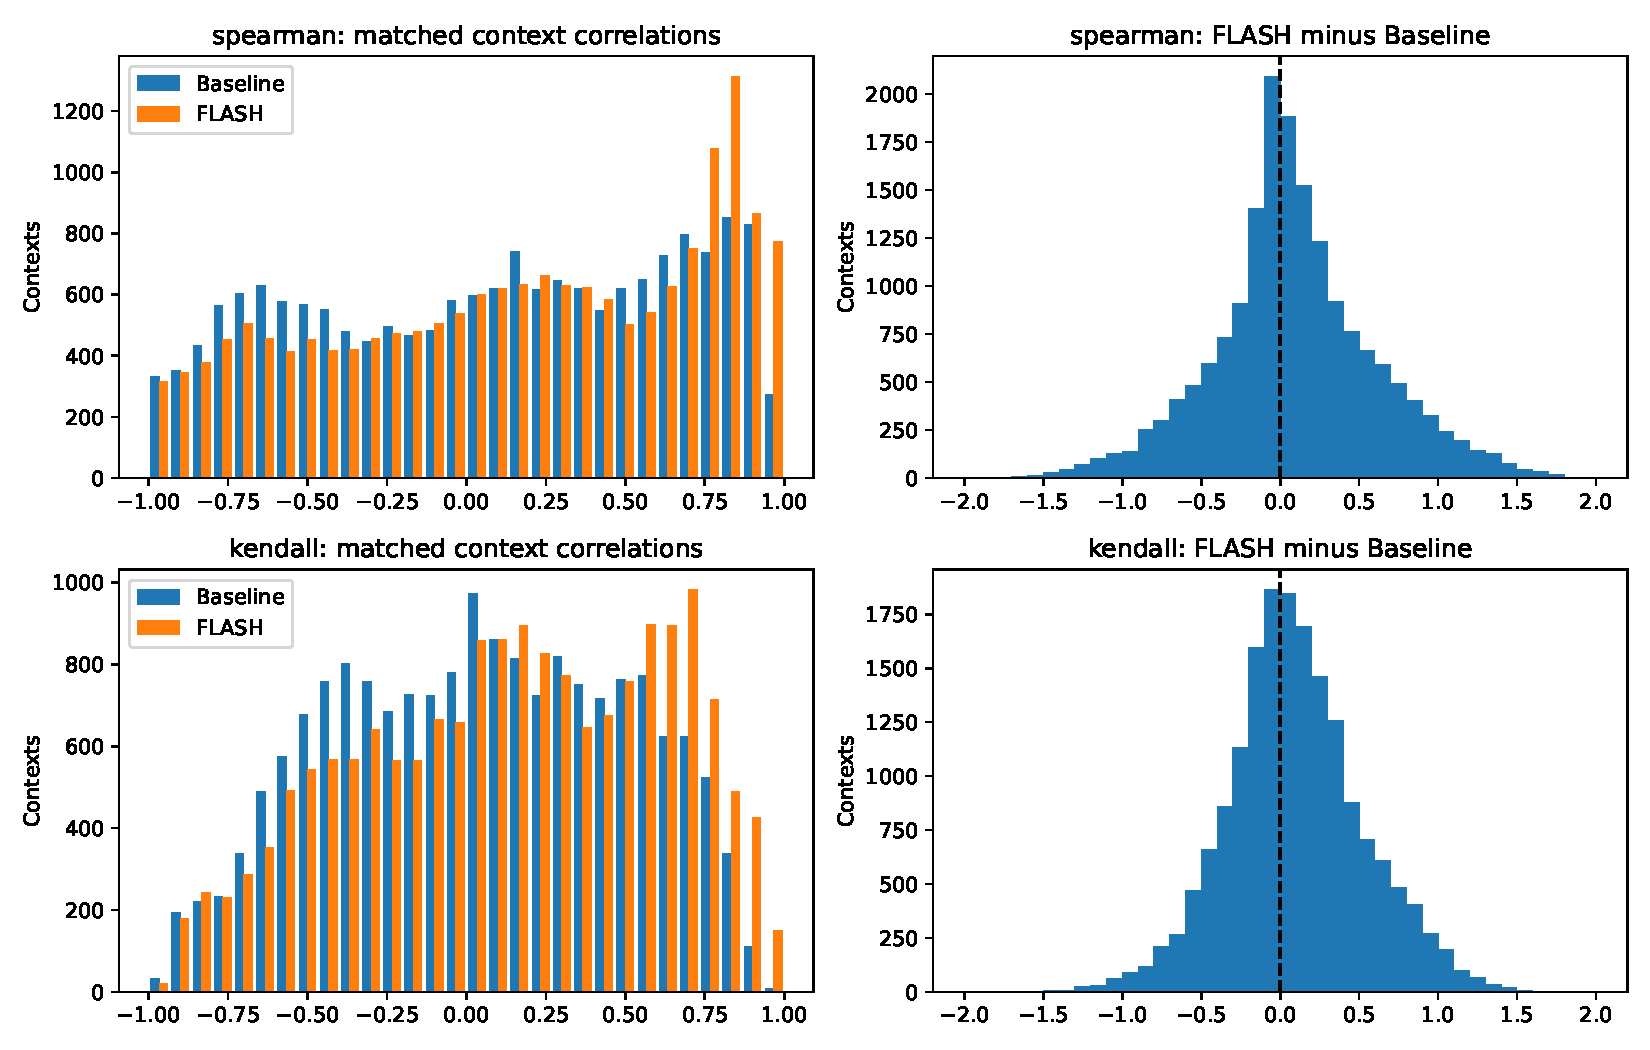
\includegraphics[width=\textwidth]{experiment/frostbite_value_seed3710_distributions.pdf}
\caption{Per-context correlation distributions for the fixed seed-3710 checkpoint pair. Left: Baseline and FLASH correlations. Right: paired FLASH-minus-Baseline differences; the dashed line marks zero. Top: Spearman; bottom: Kendall. Histogram counts are evaluated contexts, which may be temporally dependent within episodes.}
\label{fig:value_distributions}
\end{figure}

\begin{table}[!t]
\centering
\small
\caption{Direction and magnitude of changes within matched contexts. Conditional mean changes average only the contexts with positive or negative change, respectively; all differences are FLASH minus Baseline.}
\label{tab:value_context_changes}
\begin{tabular}{lrr}
\toprule
Statistic & Spearman's $\rho$ & Kendall's $\tau_b$ \\
\midrule
Higher under FLASH & 9,686 (55.60\%) & 10,001 (57.41\%) \\
Lower under FLASH & 7,733 (44.39\%) & 7,392 (42.43\%) \\
Equal & 2 (0.01\%) & 28 (0.16\%) \\
Mean change where positive & $+0.4289$ & $+0.3767$ \\
Mean change where negative & $-0.3422$ & $-0.2867$ \\
\bottomrule
\end{tabular}
\end{table}

FLASH has a higher Spearman correlation in 9,686 contexts (55.60\%), a lower correlation in 7,733 (44.39\%), and an equal correlation in two. The corresponding Kendall counts are 10,001 (57.41\%), 7,392 (42.43\%), and 28. Among contexts with a positive Spearman change, the mean increase is $0.4289$; among those with a negative change, the mean decrease has magnitude $0.3422$. The corresponding Kendall magnitudes are $0.3767$ and $0.2867$. Both the frequency and the conditional magnitude of positive changes therefore contribute to the positive overall means. These observations support improvement extending beyond a few isolated positive contexts, while also documenting substantial negative changes. Figure~\ref{fig:value_distributions} visualizes both sides of the distributions.

\subsection{Variation Across Evaluation Episodes}
For each evaluation episode $e$, we average the paired differences over its $n_e$ evaluated contexts. Table~\ref{tab:value_episode_changes} reports these episode-specific means. The mean Spearman difference is positive in 17 of 20 episodes (85\%), and the mean Kendall difference is positive in 19 of 20 (95\%). The respective ranges are $[-0.0569,\,0.2387]$ and $[-0.0224,\,0.2201]$. Thus, the positive pooled effect occurs across multiple episodes, although individual episodes contain both positive and negative context-level changes. These counts are descriptive results for the same fixed checkpoint pair, not additional training-seed replications or separate significance tests. The pooled estimates in Table~\ref{tab:value_metrics} weight contexts equally; they are not unweighted means of these 20 episode means.

\begin{table}[!t]
\centering
\small
\caption{Paired mean correlation differences by evaluation episode. IDs are zero-based collection identifiers; episode 19 is only partially observed because collection stops at 20,000 observations. Positive differences denote higher average correlation under FLASH.}
\label{tab:value_episode_changes}
\begin{tabular}{rrrr}
\toprule
Episode ID & Evaluated contexts & Mean $\Delta\rho$ & Mean $\Delta\tau_b$ \\
\midrule
0 & 783 & $-0.0006$ & $+0.0320$ \\
1 & 1,048 & $-0.0292$ & $+0.0172$ \\
2 & 957 & $+0.0343$ & $+0.0476$ \\
3 & 1,010 & $+0.0031$ & $+0.0448$ \\
4 & 861 & $+0.1738$ & $+0.1783$ \\
5 & 1,008 & $+0.1237$ & $+0.1139$ \\
6 & 907 & $+0.2387$ & $+0.2201$ \\
7 & 793 & $+0.1170$ & $+0.1174$ \\
8 & 896 & $+0.1587$ & $+0.1516$ \\
9 & 890 & $+0.1461$ & $+0.1416$ \\
10 & 896 & $+0.0800$ & $+0.1003$ \\
11 & 952 & $-0.0569$ & $-0.0224$ \\
12 & 956 & $+0.0522$ & $+0.0625$ \\
13 & 444 & $+0.1168$ & $+0.0962$ \\
14 & 848 & $+0.1453$ & $+0.1337$ \\
15 & 929 & $+0.1605$ & $+0.1551$ \\
16 & 712 & $+0.0947$ & $+0.0824$ \\
17 & 857 & $+0.1585$ & $+0.1369$ \\
18 & 1,010 & $+0.0444$ & $+0.0581$ \\
19 & 664 & $+0.0123$ & $+0.0419$ \\
\bottomrule
\end{tabular}
\end{table}

\subsection{Global Average Value Profiles}
For completeness, we also average predicted values across all contexts at each stage, $\bar v^{(m)}(k)=N^{-1}\sum_i v_i^{(m)}(k)$, and then correlate this 17-point profile with stage index. This reverses the order of averaging and correlation relative to the per-context metric and answers a different question. Baseline and FLASH respectively obtain Spearman correlations of $0.9681$ and $0.7819$, and Kendall correlations of $0.8971$ and $0.6765$, for their global profiles. These are point estimates for the averaged profiles, not additional per-context means or bootstrap intervals.

Table~\ref{tab:global_average_values} gives the complete profiles. The Baseline profile generally rises and reaches its maximum at stage 16, with some intermediate decreases. The FLASH profile peaks at stage 12, falls through stage 15, and rises again at stage 16. Thus, FLASH's higher mean per-context ordering coexists with a lower correlation of its global average profile. Neither averaging procedure implies the result of the other. Differences in raw predicted-value magnitudes are descriptive and do not by themselves establish more accurate value estimates.

\begin{table}[!t]
\centering
\small
\caption{Global average predicted value by igloo stage, using the same 17,421 contexts for both models. Bold entries mark each model's maximum.}
\label{tab:global_average_values}
\begin{tabular}{crr}
\toprule
Igloo stage & Baseline & FLASH \\
\midrule
0 & 122.5811 & 120.9317 \\
1 & 130.3185 & 134.1611 \\
2 & 135.5643 & 143.4519 \\
3 & 140.1353 & 147.9921 \\
4 & 143.5138 & 153.3676 \\
5 & 143.5928 & 161.1659 \\
6 & 142.2332 & 164.6773 \\
7 & 144.1948 & 169.2527 \\
8 & 144.3742 & 171.7132 \\
9 & 144.5918 & 175.1732 \\
10 & 146.0023 & 177.5542 \\
11 & 149.7183 & 180.4352 \\
12 & 152.8047 & \textbf{181.0360} \\
13 & 149.8857 & 174.6467 \\
14 & 148.4644 & 169.3923 \\
15 & 151.2220 & 165.3206 \\
16 & \textbf{158.5796} & 174.8477 \\
\bottomrule
\end{tabular}
\end{table}

\subsection{Interpretation and Scope}
For this checkpoint pair on Baseline-collected contexts, FLASH exhibits higher mean and median stage--value correlations, positive paired mean differences with episode-bootstrap intervals above zero, and positive episode-mean changes in most sampled episodes. The absolute correlations nevertheless remain weak on average, and a substantial fraction of contexts show lower correlations under FLASH. These findings support an average improvement in ordering for the evaluated pair, rather than uniform robustness across backgrounds.

The diagnostic tests whether predicted values increase with igloo stage under a controlled visual intervention. It does not directly measure whether latent states are disentangled, and a negative correlation can still reflect sensitivity to stage changes. Moreover, a critic predicts future return under its policy; the experiment does not establish that true expected return must increase monotonically with stage in every context. Replacing image regions also does not guarantee that each modified observation--action sequence corresponds to a realizable environment trajectory. Consequently, these results alone neither establish that spatial entanglement has been removed nor identify the cause of the evaluation-return improvements discussed in Section~\ref{subsec:exploitation_amplifier}. The background-noise probe classification experiment in Appendix~\ref{sec:appendix_noise_robustness_flash} is a separate diagnostic and is not pooled with this value analysis.

\section{Detailed Probing Experiments and Robustness Analysis}
\label{sec:appendix_detailed_probing}
This section provides the comprehensive experimental setup and extended results for the probing and noise injection experiments summarized in Section~\ref{subsec:probing_latent}.

\subsection{Preliminary Observation: The Cosine Similarity Clue}
To formally investigate whether the encoder successfully captures functionally critical, yet small and static elements, we designed a motivating experiment. Instead of a single comparison, we generated two comprehensive sets of images by fixing the background to be perfectly identical and replacing only the diver regions to vary the target elements: one varying the number of collected divers at the bottom area (from 0 to 6), and another varying the position of a single diver on the sea area. We then extracted their latent states and computed the pairwise cosine similarities.

\begin{figure}[!t]
\centering
\begin{minipage}{0.48\textwidth}
  \centering
  \includegraphics[width=\linewidth]{heatmap/diver_count.jpg}
  \caption{Cosine Similarity: Diver Count (0-6)}
  \label{fig:heatmap_count}
\end{minipage}\hfill
\begin{minipage}{0.48\textwidth}
  \centering
  \includegraphics[width=\linewidth]{heatmap/diver_location.jpg}
  \caption{Cosine Similarity: Diver Position}
  \label{fig:heatmap_position}
\end{minipage}
\caption{Cosine similarity heatmaps of latent states in Seaquest. The structured similarity patterns suggest sensitivity to changes in the target regions. These patterns motivate evaluating whether supervised probes can predict the corresponding task variables from latent states.}
\label{fig:heatmaps}
\end{figure}

As shown in Figure~\ref{fig:heatmaps}, both heatmaps reveal distinct structural patterns rather than a uniform similarity of 1.0. For the diver count (left), states with similar counts exhibit high cosine similarity ($0.93$--$0.98$), while states with larger count differences drop as low as $0.86$. For the diver position (right), we fixed the submarine at the center and moved a single diver from the far left edge to just left of the submarine; as displacement increases, the similarity degrades down to $0.63$. These patterns suggest sensitivity to the controlled visual changes, motivating our subsequent probing analysis. They do not by themselves establish that a probe can accurately predict the underlying task variables from latent states. If latent sampling is used, stochastic variation must also be controlled when interpreting these differences.

\subsection{Probing the Latent Space}
\label{subsec:appendix_probing_latent}
To examine whether a lightweight MLP can predict diver counts and positions from the latent state $z$, we conducted a probing experiment on the Seaquest environment. We used an encoder trained in a run that never encountered states with 4 to 6 collected divers. We froze this encoder and trained the MLP to predict ground-truth RAM states directly from $z$. To evaluate count prediction for states absent from encoder training, we used the frozen encoder to extract latents from manually collected demonstrations containing 4 to 6 collected divers. We combined these latents with those from newly collected rollouts from the same run (entirely independent of the encoder's original replay buffer) to construct the probing dataset. The probing MLP was trained on labeled examples spanning all counts from 0 to 6, including the demonstrations with 4 to 6 divers.

First, for classifying the number of collected divers at the bottom (0 to 6), the probe achieved an overall accuracy of 99.6\%. The MLP also predicted counts of 4 to 6 with $>93\%$ accuracy after supervised training on examples that included these counts, using latent representations from the frozen encoder. These results suggest that the representations support supervised count prediction even for count values absent from encoder training.

Second, we tasked the probe with predicting the exact $(x, y)$ coordinates of multiple dynamic divers swimming on the screen. Since up to 4 divers can appear simultaneously, simply assigning fixed output slots to specific lanes introduces a structural bias. To ensure a strictly fair evaluation, we formulated this as a Set Prediction problem and employed a Permutation-Invariant Bipartite Matching Loss, inspired by modern object detection frameworks like DETR. The MLP was forced to output an unordered set of 4 object predictions (presence probability and coordinates), which were then optimally matched to the ground-truth divers via Hungarian matching. Using this rigorous setup, the probe achieved $92.4\%$ accuracy for predicting diver presence, and an average spatial error of $12.44$ pixels for pinpointing their precise $(x, y)$ locations. These results show that the MLP can use latent states to predict object presence and location on the evaluated data, despite poor visual reconstruction. They do not establish complete information preservation or a disentangled representation.

It is important to acknowledge that the Atari 2600 emulator exhibits an intrinsic temporal and spatial misalignment between the internal RAM state and the rendered visual frame. For instance, when the submarine collects a diver, the RAM counter increments immediately, but the visual rendering of the diver often persists on the screen for an additional frame before being visually absorbed. Similarly, minor discrepancies exist between the exact pixel locations of moving sprites and their corresponding RAM values due to the Atari hardware's rendering cycle. These hardware-level asynchronies impose an irreducible upper bound on probing accuracy. These mismatches may contribute to the residual probing errors (see Appendix \ref{sec:appendix_ram_misalignment} for visual examples). However, the present experiments do not quantify their contribution or rule out information loss and limitations of the probe as additional sources of error.

\subsection{Robustness to Spatial Noise: Assessing Background Sensitivity}
DIAMOND \citep{alonso2024diffusion} notes that compression into discrete latent representations may lose task-relevant visual details and reports visual inconsistencies between frames imagined by IRIS. Our analysis separately examines whether supervised probes can predict selected task variables from latent states and whether their predictions are sensitive to changes outside the target region. To assess this background sensitivity, we injected extreme random uniform noise into the background spaces of the original observations, leaving only the bounding box of the target objects perfectly intact. We conducted this experiment across two distinct domains: classifying the number of bottom divers in Seaquest, and classifying the igloo construction stages (0--16 blocks) in Frostbite. (For full details on the MLP training procedure and rigorous evaluation setup, see Section~\ref{subsec:appendix_probing_latent}.)

To assess sensitivity to changes outside the target region, we evaluated the probing MLP on these noise-injected images and observed a substantial accuracy drop. As detailed in Table~\ref{tab:per_class_noise}, in Seaquest, accuracy dropped from $99.6\%$ (clean) to $68.1\%$ (effectively random chance, as it converged to predicting the majority class). We observed an even more dramatic collapse in Frostbite (Table~\ref{tab:per_class_noise_frostbite}), where the accuracy for predicting the igloo stage fell from a pristine $99.2\%$ down to $27.7\%$ upon background noise injection. These results show that the encoder--probe pipeline is sensitive to background corruption, consistent with spatial entanglement. However, because extreme noise introduces a substantial distribution shift, the experiment does not distinguish encoder sensitivity from limitations in probe generalization, nor establish that spatial entanglement is the sole explanation.

\begin{table}[!t]
    \centering
    \caption{Per-class classification accuracy for bottom diver counting in Seaquest. The clean setting uses the uncorrupted $64 \times 64$ observation, while the noisy setting injects uniform random noise everywhere except the tight bounding box containing the divers. The drop in minority class accuracy indicates sensitivity of the encoder--probe pipeline to background corruption.}
    \label{tab:per_class_noise}
    \begin{tabular}{crrr}
        \toprule
        \textbf{Diver Count} & \textbf{Samples ($n$)} & \textbf{Clean Accuracy (\%)} & \textbf{Noisy Accuracy (\%)} \\
        \midrule
        0 & $39,767$ & $99.8$ & $96.9$ \\
        1 & $17,003$ & $99.3$ & $9.8$ \\
        2 & $1,374$ & $95.8$ & $0.0$ \\
        3 & $260$ & $95.4$ & $0.0$ \\
        4 & $146$ & $95.9$ & $0.0$ \\
        5 & $417$ & $96.9$ & $0.0$ \\
        6 & $110$ & $90.9$ & $0.0$ \\
        \midrule
        \textbf{Overall} & \textbf{59,077} & \textbf{99.5} & \textbf{68.1} \\
        \bottomrule
    \end{tabular}
\end{table}

\begin{table}[!t]
    \centering
    \caption{Per-class classification accuracy for igloo construction stages (0--16) in Frostbite. Similar to Seaquest, injecting background noise outside the igloo bounding box severely degrades the probing accuracy, indicating sensitivity of the encoder--probe pipeline to changes outside the target region.}
    \label{tab:per_class_noise_frostbite}
    \begin{tabular}{crrr}
        \toprule
        \textbf{Igloo Stage} & \textbf{Samples ($n$)} & \textbf{Clean Accuracy (\%)} & \textbf{Noisy Accuracy (\%)} \\
        \midrule
        0 & $153$ & $99.3$ & $0.0$ \\
        1 & $26$ & $96.2$ & $0.0$ \\
        2 & $25$ & $92.0$ & $0.0$ \\
        3 & $28$ & $100.0$ & $0.0$ \\
        4 & $77$ & $98.7$ & $0.0$ \\
        5 & $54$ & $100.0$ & $0.0$ \\
        6 & $159$ & $100.0$ & $0.6$ \\
        7 & $377$ & $99.7$ & $75.6$ \\
        8 & $95$ & $98.9$ & $0.0$ \\
        9 & $91$ & $98.9$ & $0.0$ \\
        10 & $121$ & $100.0$ & $0.0$ \\
        11 & $120$ & $98.3$ & $0.0$ \\
        12 & $47$ & $97.9$ & $0.0$ \\
        13 & $89$ & $97.8$ & $0.0$ \\
        14 & $28$ & $92.9$ & $0.0$ \\
        15 & $70$ & $100.0$ & $0.0$ \\
        16 & $294$ & $100.0$ & $77.6$ \\
        \midrule
        \textbf{Overall} & \textbf{1,854} & \textbf{99.2} & \textbf{27.7} \\
        \bottomrule
    \end{tabular}
\end{table}

Taken together, the cosine similarity patterns suggest sensitivity to target-region changes, and the high clean probing accuracy shows that supervised probes can accurately predict the evaluated task variables from latent states. These results support the claim that lightweight encoders can retain task-relevant information despite poor reconstruction, while leaving open whether other information is lost and how robustly the retained information generalizes across observation distributions.

These findings motivate a downstream intervention without requiring a universal claim of information preservation. If task-relevant information is available but not effectively used by the Actor-Critic, targeted retrieval may improve its utilization. FLASH explores this possibility by retrieving structurally similar historical contexts and injecting them into the same training batch. We treat improved utilization of the available representations as the motivating hypothesis, rather than claiming that probing alone proves the cause of policy learning failures.

\section{Preliminary Behavioral Observations in DRAMA on Seaquest}
\label{sec:appendix_ac_bottleneck}
This appendix documents the preliminary observation motivating the downstream optimization question in the Introduction. Under the same DRAMA training configuration, we observed average evaluate scores of approximately 600 and 1,500 on Seaquest. In the inspected behavior, the lower-scoring run died in collisions while hunting, whereas the higher-scoring run continued hunting until oxygen depletion. Neither exhibited surfacing with collected divers. These are selected observations, not an estimate of the frequency of either behavior across training runs.

\subsection{Trajectory Evidence}
\todo{Add series of figure with two rows of original-resolution Seaquest frames, one per inspected run. Show representative hunting behavior and frames immediately before and after a death, with environment steps, scores, and the oxygen gauge visible. Identify the source episode for each row. State in the caption that these are selected examples, and distinguish a life loss from the end of an episode. Do not treat a few frames as evidence that diver-return behavior never occurred.}

\subsection{Interpretation and Limitations}
The observed score difference was accompanied by a difference in how long hunting behavior was sustained and how the inspected behavior ended, without observed success in returning divers. It therefore motivates asking whether more effective use of available experiences could improve control with a lightweight encoder architecture. It does not establish that the agent lacks diver-related information, that the learned representations are identical across runs, or that Actor-Critic optimization alone explains the score difference. Exploration, collected data, and learned encoder and world-model parameters can differ even under the same training configuration.

We use this observation as motivation for FLASH, rather than as evidence of its effectiveness or a causal diagnosis of the performance gap. FLASH targets reuse of experiences already encountered; whether it improves aggregate performance or reliability requires evaluation across runs. Likewise, a gap between the best training episode and average evaluation return would not by itself isolate an optimization failure, because the two statistics differ in selection and may also differ in evaluation conditions.

\section{Ablation Studies on Triggering and Retrieval}
\label{sec:appendix_ablation_studies}
To isolate and validate the impact of the core components introduced in FLASH, we conducted rigorous ablation studies. The summarized results discussed in Section \ref{subsec:ablation_main} are elaborated below.

\subsection{Ablation 1: The Role of Retrieval (In-batch Injection)}
In this setting, we preserve the exact triggering condition of FLASH ($\text{ReLU(TD-error)} \times \text{Softplus(Value Difference)}$) but completely disable the subsequent retrieval mechanism. When a pivotal anchor is triggered, it is injected into the training batch alone, without pulling in structurally similar historical states from the hash buckets. The observed performance drop supports the utility of retrieving structurally similar historical contexts in addition to the selected anchor. In the evaluated setting, anchor injection alone does not reproduce the performance of the full method.

\subsection{Ablation 2: Value Difference vs. Absolute Value}
Here, we replace the temporal value difference ($|V(s_t) - V(s_{t-1})|$) in the triggering condition with the absolute state value ($V(s_t)$). Using the absolute value causes the anchor mechanism to trigger continuously once the agent enters a high-reward phase, leading to redundant sampling and a loss of focus. The temporal difference ensures that FLASH specifically targets the pivotal moments of value spikes, focusing anchor selection on changes in the estimated value.

\subsection{Ablation 3: Multiplicative vs. Additive Combination}
In this ablation, we substitute our multiplicative trigger condition with an additive linear combination, similar to prior works like HVPER: $\lambda \cdot \text{TD-error} + (1-\lambda) \cdot \text{Value Difference}$. The additive approach is prone to false positives; a massive TD-error caused by environmental noise can trigger an anchor even if there is zero value difference. Our multiplicative formulation effectively acts as a logical AND gate, suppressing these noisy false positives and ensuring that only truly pivotal learning moments are retrieved.

\todo{Include comprehensive tables and graphs detailing the specific quantitative performance metrics across the evaluated environments for these three ablations.}

\section{Extended Related Work}
\label{sec:appendix_related_work}
This section expands the background and comparisons summarized in Section~\ref{sec:related}.

\subsection{Latent World Models and Imagination-Based Learning}
Latent world models encode visual observations into compact states and learn dynamics that generate imagined trajectories for policy and value learning. Dreamer \citep{hafner2019dream} and DreamerV2 \citep{hafner2020mastering} established Actor-Critic learning in latent imagination. STORM \citep{zhang2023storm}, the primary base agent in our experiments, combines stochastic latent states with Transformer-based dynamics. DRAMA \citep{wang2025drama} explores Mamba-based dynamics to improve sample and parameter efficiency. FLASH operates within this setting by augmenting the historical contexts used to initialize imagined trajectories, while retaining the underlying encoder and world-model architectures.

\subsection{Representation Learning and Visual Fidelity}
Learning compact representations that retain information relevant for control is a central challenge in visual RL \citep{hafner2019learning}. Several methods address this through representation-learning objectives. CURL \citep{laskin2020curl} introduces contrastive unsupervised learning, while SPR \citep{schwarzer2020data} uses temporal predictive consistency to learn invariant representations. ATC \citep{stooke2021decoupling} decouples representation learning from policy optimization. DreamerPro \citep{deng2022dreamerpro} adopts reconstruction-free, prototypical representations. These approaches motivate examining both what information a representation retains and how downstream learning uses it.

DIAMOND \citep{alonso2024diffusion} replaces the discrete latent bottleneck with a diffusion-based world model to preserve complex visual details. This approach emphasizes visual fidelity, with additional computation associated with generative modeling. FLASH explores a complementary intervention: targeted reuse of experience during Actor-Critic training with the existing lightweight encoder. It does not require replacing the representation-learning objective or introducing a heavier generative model.

\subsection{Episodic Memory for Value Estimation and Control}
Model-Free Episodic Control (MFEC; \citealp{blundell2016model}) stores the highest observed returns for state-action pairs and uses nearest-neighbor lookup to estimate values for unseen states. Neural Episodic Control (NEC; \citealp{pritzel2017neural}) combines learned state embeddings with a differentiable neural dictionary for rapid value estimation. EVA \citep{hansen2018fast} retrieves similar historical experiences to adjust and augment parametric value estimates. ERLAM \citep{zhu2020episodic} structures episodic memory through associative graphs for trajectory propagation, while subsequent work incorporates state abstraction \citep{li2023neural}.

The distinction relevant to FLASH is how retrieved experience enters learning. Rather than using retrieved returns directly as a component of value estimation, FLASH searches hash buckets for structurally similar contexts around selected anchors. These contexts enter the same imagination batch and support training with the existing Actor-Critic objectives. Hash indexing also avoids the need for a full nearest-neighbor search or an explicit associative graph.

\subsection{Priority Signals and Anchor Selection}
Prioritized Experience Replay uses TD-error to prioritize transitions \citep{schaul2015prioritized}. Other approaches incorporate value-related signals \citep{cao2019high} or model-based curiosity \citep{kauvar2023curious}. Sequence-level methods extend prioritization beyond individual transitions \citep{karimpanal2018experience, brittain2019prioritized}, and actor-critic-specific methods tailor replay priorities to the learning objectives \citep{saglam2023actor}. Prioritized Sweeping \citep{moore1993prioritized} uses changes in value estimates to schedule backups.

FLASH's anchor score differs in two design choices. First, it uses the signed temporal difference between consecutive state values, $\Delta V_t = V(s_t)-V(s_{t-1})$, rather than absolute state value. This differs from the before-and-after-update value change used in Prioritized Sweeping: the two signals compare different states along a trajectory and different estimates of a state, respectively. Second, FLASH combines normalized TD-error and temporal value difference multiplicatively through ReLU and softplus, rather than the additive combination discussed for HVPER \citep{cao2019high}. The ReLU factor requires above-average TD-error for a positive score, while the softplus factor modulates the score according to value change. The exact formulation is given in Section~\ref{subsec:flash_retrieval}. Anchor selection is followed by retrieval of related contexts, whose contribution beyond anchor injection alone is evaluated in Appendix~\ref{sec:appendix_ablation_studies}.

\end{document}
